\chapter{Team 1 Agent Design}\label{team_1_agent_design}

\section{Overview}

The following chapter presents the design and implementation of Team 1's agent. The agent presented agent seeks to imitate important parts of human behaviour such as social status, social networks, selfishness, forgiveness and learning from experiences. At the end of the chapter, it will be shown that by using these concepts, the agent produces better collective outcomes over agents performing random actions.

\section{Core Structure}
Figure \ref{fig:agent_structure} presents a high-level overview of the structure and operation of our agent. In broad terms, the agent contains three elements which impact decision-making. These elements are:
\begin{enumerate}
  \item Social capital: Socially constructed resources which facilitate cooperation to solve collective problems.
  \item Selfishness: A continuously updated variable dictating to what degree an  agent prioritizes its own utility over the social welfare of the group when making decisions. 
  \item Q-functions: Functions learned through reinforcement learning which estimate the impact of actions given the current game state.
\end{enumerate}
In addition to these components which are inherent to the agent, the current state of the game, known as the \emph{environment}, also influences decisions. Exactly how each component is used in the decision making process varies between different types of decisions, and social capital, selfishness and q-functions are not all used for every decision. The specific decision process for each type of decision will be discussed in greater detail in \ref{}.

%However, a general decision flow can be as follows: The agent takes in the current game state and passes it through a set of Q-functions. The Q-functions return the expected utility of each action to the collective and to the agent itself. Based on its current selfishness value, the agent aggregates the two utility values into a single value for each action.   Generally, the decision flow 

After each round of the game, the agents will update their internal state. Specifically, the agents will update their selfishness based on the current environment and the social capital of agents, while the social capital will be updated based on the actions of agents. The social capital is also updated every time an agent receives a message from an agent in their network. All of these update mechanisms are indicated by red arrows in Figure \ref{fig:agent_structure}. As can be seen, there is no arrow feeding back to the Q-functions as they do not update over the course of a single game. Instead, the Q-functions are updated based on the results from a series of games. However, as will be discussed later, the updating of selfishness values does still permit the agents to learn from experiences during a game.

\begin{figure}[!h]
    \centering
    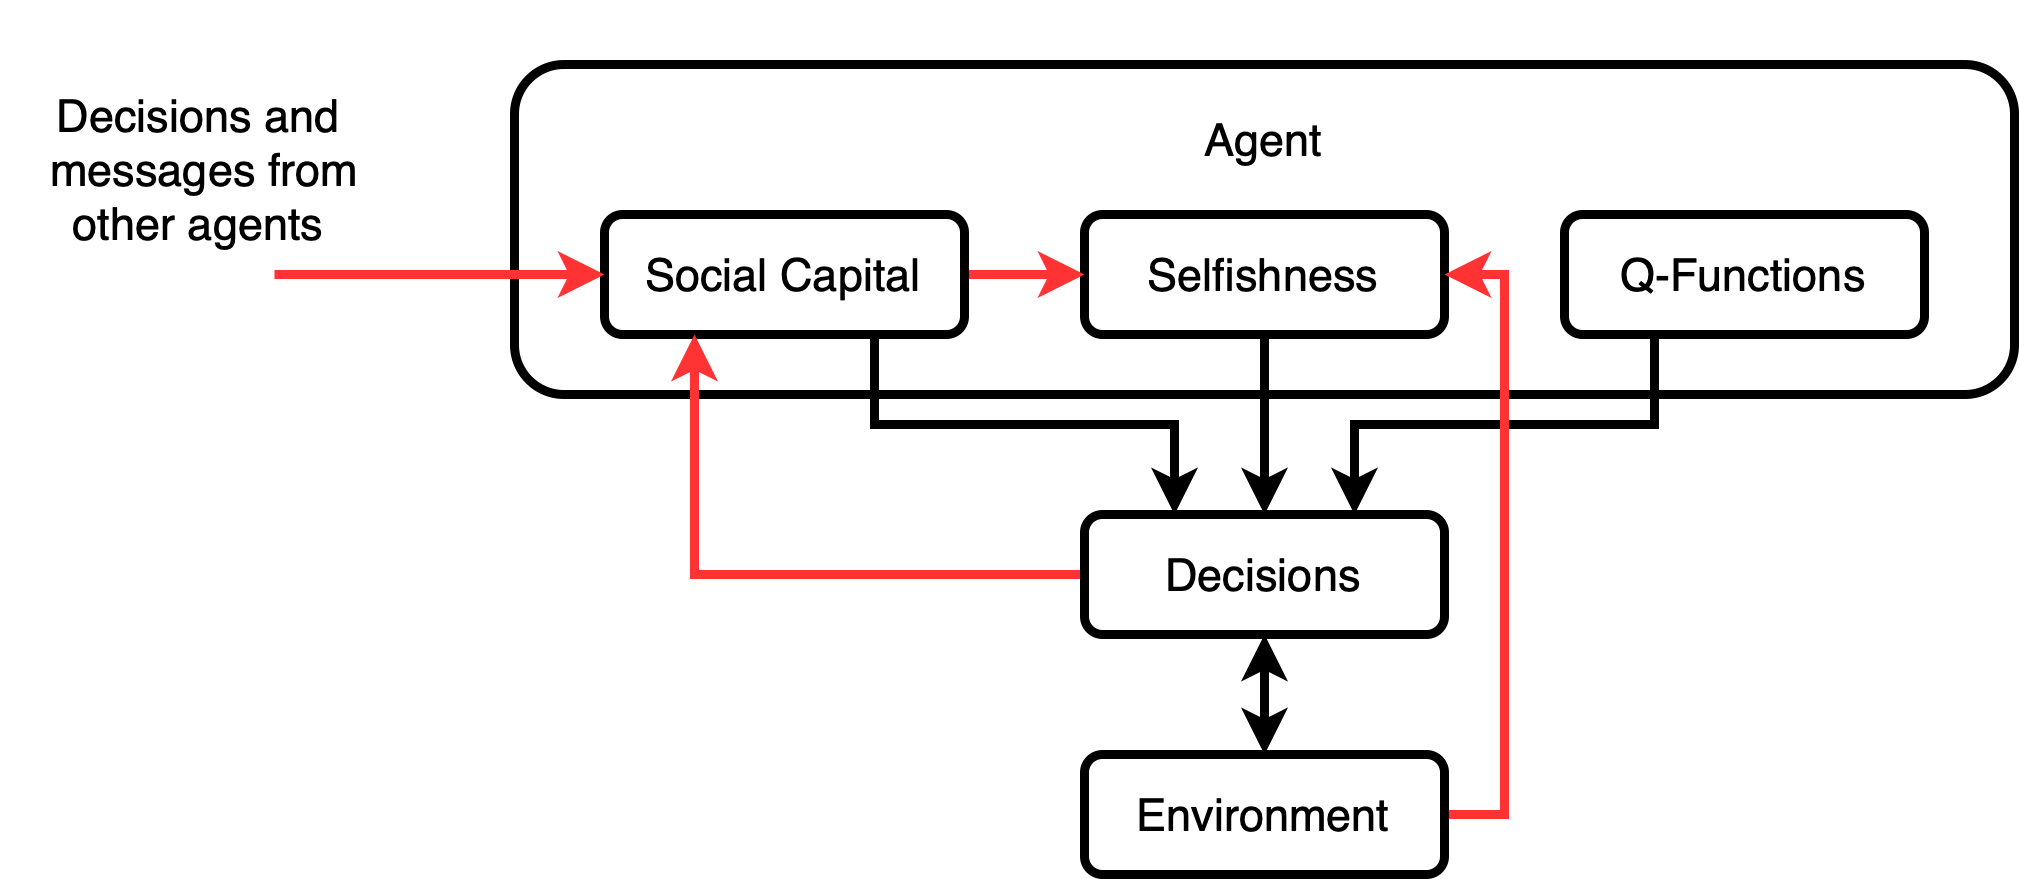
\includegraphics[width=0.75\linewidth]{004_team_1_agent_design/images/agent_structure.png}
    \caption{Overview of agent structure.}
    \label{fig:agent_structure}
\end{figure}

\section{Social Capital}

The core concept underlying the design of the agent is the idea of social capital. The exact definition of the term "social capital" varies between works, but can be summarized as "an 'umbrella term' for a range of socially constructed conceptual resources that help people coordinate expectations and self-organise."\cite{pitt}. Several forms of social capital have been identified and defined. Our work on social capital is mostly related to those forms laid out by Elinor Ostrom and T. K. Ahn in their 2007 paper "The meaning of social capital and its link to collective action". \cite{ostrom-ahn} In their paper, Ostrom and Ahn identified three forms of social capital. These were \emph{Institutions}, \emph{Networks} and \emph{Trustworthiness}. In addition to the forms of social capital presented by Ostrom and Ahn, we have as a team identified another form of social capital elected to call \emph{Honour}. With \emph{Honour} we refer to the human tendency to want to return a favour, or similarly, our appetite for revenge. A more comprehensive definition of honour is given in section \ref{subsection:honour}. 

In order to use social capital to promote cooperation, it must be used as part of a framework where the actions of an agent impact their social capital and where the social capital is used to make informed decision on whether or not to cooperate with other agents. For our agent, we used a similar framework to that presented by Petruzzi, Pitt, and Busquets\cite{complexity_reduction}. An overview diagram of this framework is presented in Figure \ref{fig:social_capital_framework}. In this framework events coming the environment are translated into social capital information which is passed to internal update functions for calculating metrics for each type of social capital. The social capital decision module uses the social capital metrics to calculate a value from 0 (no cooperation) to 1 (full cooperation) indicating whether an agent should cooperate or not. Implementing this framework for a simple cooperation game, Petruzzi et al. were able to achieve better performance than the dominant strategy given by game theory analysis. 

\begin{figure}[!h]
    \centering
    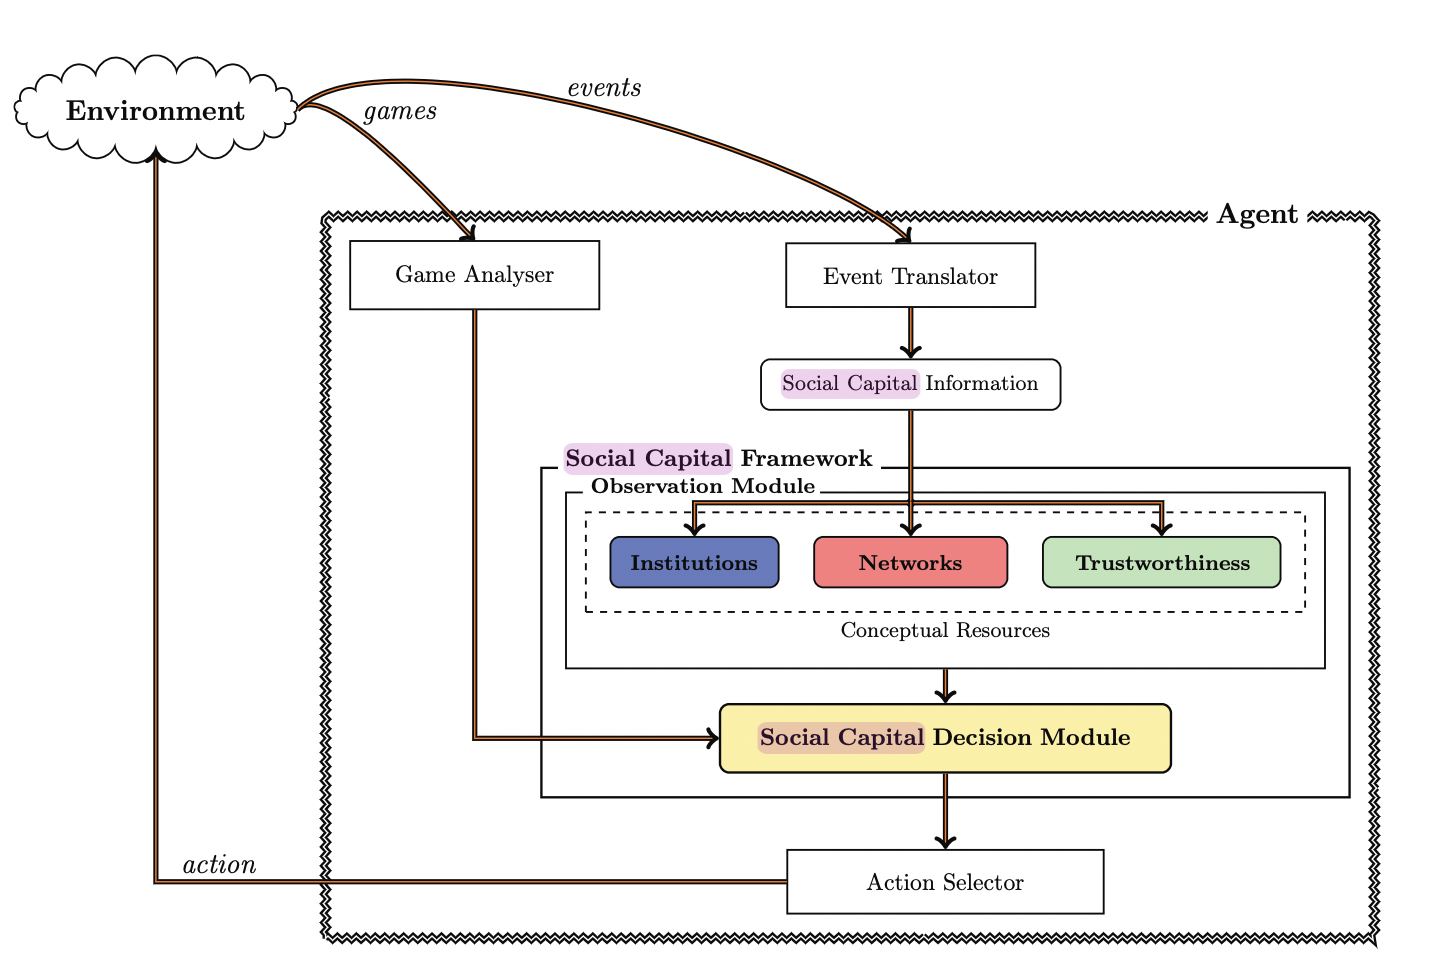
\includegraphics[width=0.75\linewidth]{004_team_1_agent_design/images/socialcapitalframework.png}
    \caption{Framework for a social capital system.\cite{pitt}}
    \label{fig:social_capital_framework}
\end{figure}

To apply the framework to the Escape the Dark Pit(t) game, we used a slightly different implementation than Petruzzi et al. used for their cooperation game. Most prominently, we simplified the stored metrics on social capital down to a single number between -1 and 1 for each form of social capital. We also simplified the social capital decision module by removing the possibility of weighting social capital indicators differently, reducing the decision module to a simple summing function. 

The specific implementation is as follows. Each agent has a member variable $socialCaptial$ which is a map between agent ids and an array with 4 values. From index 0 to index 3, this array holds values describing the social capital related to institutions, networks, trustworthiness and honour respectively for the agent with the specified agent id. Each agents $socialCapital$ map contains an array for every single agent in the game, including themselves. The array values are bounded between -1 and 1, where a higher number indicates higher social capital. When an agent is created, all the array values are initialized as 0. This is a neutral state in which no agent has a negative nor positive impression of another agent. Throughout the game the array values for each agent will change based on their actions and messages received about them. In general, if an agent does a non-cooperative actions the array values will decrease and become negative, and inversely cooperative actions will give positive array values. As such, agents will try to reward other agents for which their $socialCapital$ map indicates positive social capital and punish those who have negative social capital.

The following subsections go into detail regarding the implementation of each form of social capital.

\subsection{Institutions}

In their 2007 paper Ostrom and Ahn defined institutions as "prescriptions that specify what actions (or outcomes) are required, prohibited, or permitted, and the sanctions authorized if the rules are not followed" \cite{ostrom-ahn}. With our $Institutions$ social capital value we seek to provide a metric on how likely an agent is to follow these prescriptions and cooperate within institutions. 

During a game our agents place the following expectation on the interaction of other agents with institutions:

\begin{enumerate}
    \item If the leader makes a fight proposal, all agents should follow that proposal.
    \item If the leader makes a loot allocation proposal, all agents should follow that proposal.
\end{enumerate}

Failing to comply with any of these two expectations will lead to an agent being labelled as a defector. Once labelled as a defector, an agent's social capital value for institutions will for the rest of the game be given a base value of -1. As such, even deviating from the required action once will lead to a negative perception for the entirety of the remaining game. This is similar to a grim trigger strategy for cooperation. The reason why we elected to have defecting in even a single round negatively effect the social capital of an agent for all remaining rounds is due to the limitation on available information from the game. In its current version, the list of defectors which the game makes available to agent has the same type of static behaviour where defecting once will lead to an agent being labelled a defector for the rest of the game.

In order to increase their $Institutions$ social capital value agents must demonstrate their cooperation within institutions. For our agents there is just a single way of doing this: being elected leader. For as long as an agent is the leader, they will get a temporary boost of +1 to their $Institutions$ social capital value. Originally, agents tendency to sanction defectors was also planned to impact their social capital. In this case, doing actions which punish defectors such as voting against them in elections and not trading with them would yield positive social capital. Inversely, voting for defectors or trading with them would yield negative social capital. However, this was in practice found to be hard to implement, and has been left as a possible future extension.

\subsection{Networks}

The $Networks$ social capital value is a measure of an agent's reputation among other agents. Specifically, the $Networks$ value tries to estimate the average social capital perception of the given agent among the other agents in the game. 

 !!!!
SHERWIN here you need to talk about:
- How an agents $Networks$ value is updated
- What messages we send between agents
- When we send messages between agents
- The connections between agents
 !!!

\subsection{Trustworthiness}

\subsection{Honour}
\label{subsection:honour}

\section{Forgiveness}

\section{Selfishness}

Starts at a random value, as such we get agents with differing behaviour. Hope is that the social capital framework through sanctions encourages cooperative behaviour and thus low selfishness in the group as a whole.

Weighting of how much agent prioritises its own performance over the performance of the group as a whole.

\subsection{Impact on Decision Making}

\subsection{Updating Selfishness}


\section{Sanctions}

\subsection{Exclusion from Trading}

\subsection{Elections}

\section{Q-learning}

\section{Experiments}
do not use HP-pool as it is OP

\section{Agent Performance}

\section{Conclusion}